
% RECOMMENDED %%%%%%%%%%%%%%%%%%%%%%%%%%%%%%%%%%%%%%%%%%%%%%%%%%%
\documentclass[graybox]{svmult}

% choose options for [] as required from the list
% in the Reference Guide

\usepackage{mathptmx}       % selects Times Roman as basic font
\usepackage{helvet}         % selects Helvetica as sans-serif font
\usepackage{courier}        % selects Courier as typewriter font
\usepackage{type1cm}        % activate if the above 3 fonts are
                            % not available on your system
%
\usepackage{makeidx}         % allows index generation
\usepackage{graphicx}        % standard LaTeX graphics tool
                             % when including figure files
\usepackage{multicol}        % used for the two-column index
\usepackage[bottom]{footmisc}% places footnotes at page bottom

% see the list of further useful packages
% in the Reference Guide

\makeindex             % used for the subject index
                       % please use the style svind.ist with
                       % your makeindex program

%%%%%%%%%%%%%%%%%%%%%%%%%%%%%%%%%%%%%%%%%%%%%%%%%%%%%%%%%%%%%%%%%%%%%%%%%%%%%%%%%%%%%%%%%
\usepackage{multirow}

\begin{document}

\title*{Tumores neuro-epiteliais de baixo grau}
% Use \titlerunning{Short Title} for an abbreviated version of
% your contribution title if the original one is too long
\author{Francisco Hélder Cavalcante Félix e Juvenia Bezerra Fontenele}
% Use \authorrunning{Short Title} for an abbreviated version of
% your contribution title if the original one is too long
\institute{Francisco Hélder Cavalcante Félix \at Centro Pediátrico do Câncer, Hospital Infantil Albert Sabin, R. Alberto Montezuma, 350, 60410-780, Fortaleza - CE \email{fhcflx@outlook.com}
\and Juvenia Bezerra Fontenele \at Faculdade de Farmácia, Odontologia e Enfermagem, Universidade Federal do Ceará, R. Alexandre Baraúna, 949, 60430-160, Fortaleza - CE %\email{juvenia.fontenele@gmail.com}
}
%
% Use the package "url.sty" to avoid
% problems with special characters
% used in your e-mail or web address
%
\maketitle

\abstract{Esse grupo inclui os astrocitomas, oligodendrogliomas, gangliogliomas e tumores neurogliais mistos ou variantes (grupos IIIa, b e d da CICI 3). A denominação de baixo grau refere-se à classificação da OMS para tumores do sistema nervoso central, a qual divide as neoplasias em 4 grupos, baseada em critérios histológicos. A classificação da OMS para tumores do sistema nervoso central constitui uma “escala de malignidade”, mais do que um esquema de estadiamento convencional. Os tumores classificados como Grau I ou II são coletivamente denominados tumores de baixo grau de malignidade, enquanto aqueles classificados como Grau III ou IV são designados tumores de alto grau de malignidade. Os tumores de baixo grau são comumente tratados apenas cirurgicamente, com elevados índices de cura e sobrevida prolongada. Tumores astrocíticos e oligodendrogliais de baixo grau têm bom prognóstico associado à ressecção cirúrgica como única terapia. Todavia, a possibilidade de ressecção cirúrgica completa varia muito de acordo com o sítio tumoral.}

\section{Gliomas de baixo grau}
\begin{center}
\begin{figure}[!htb]
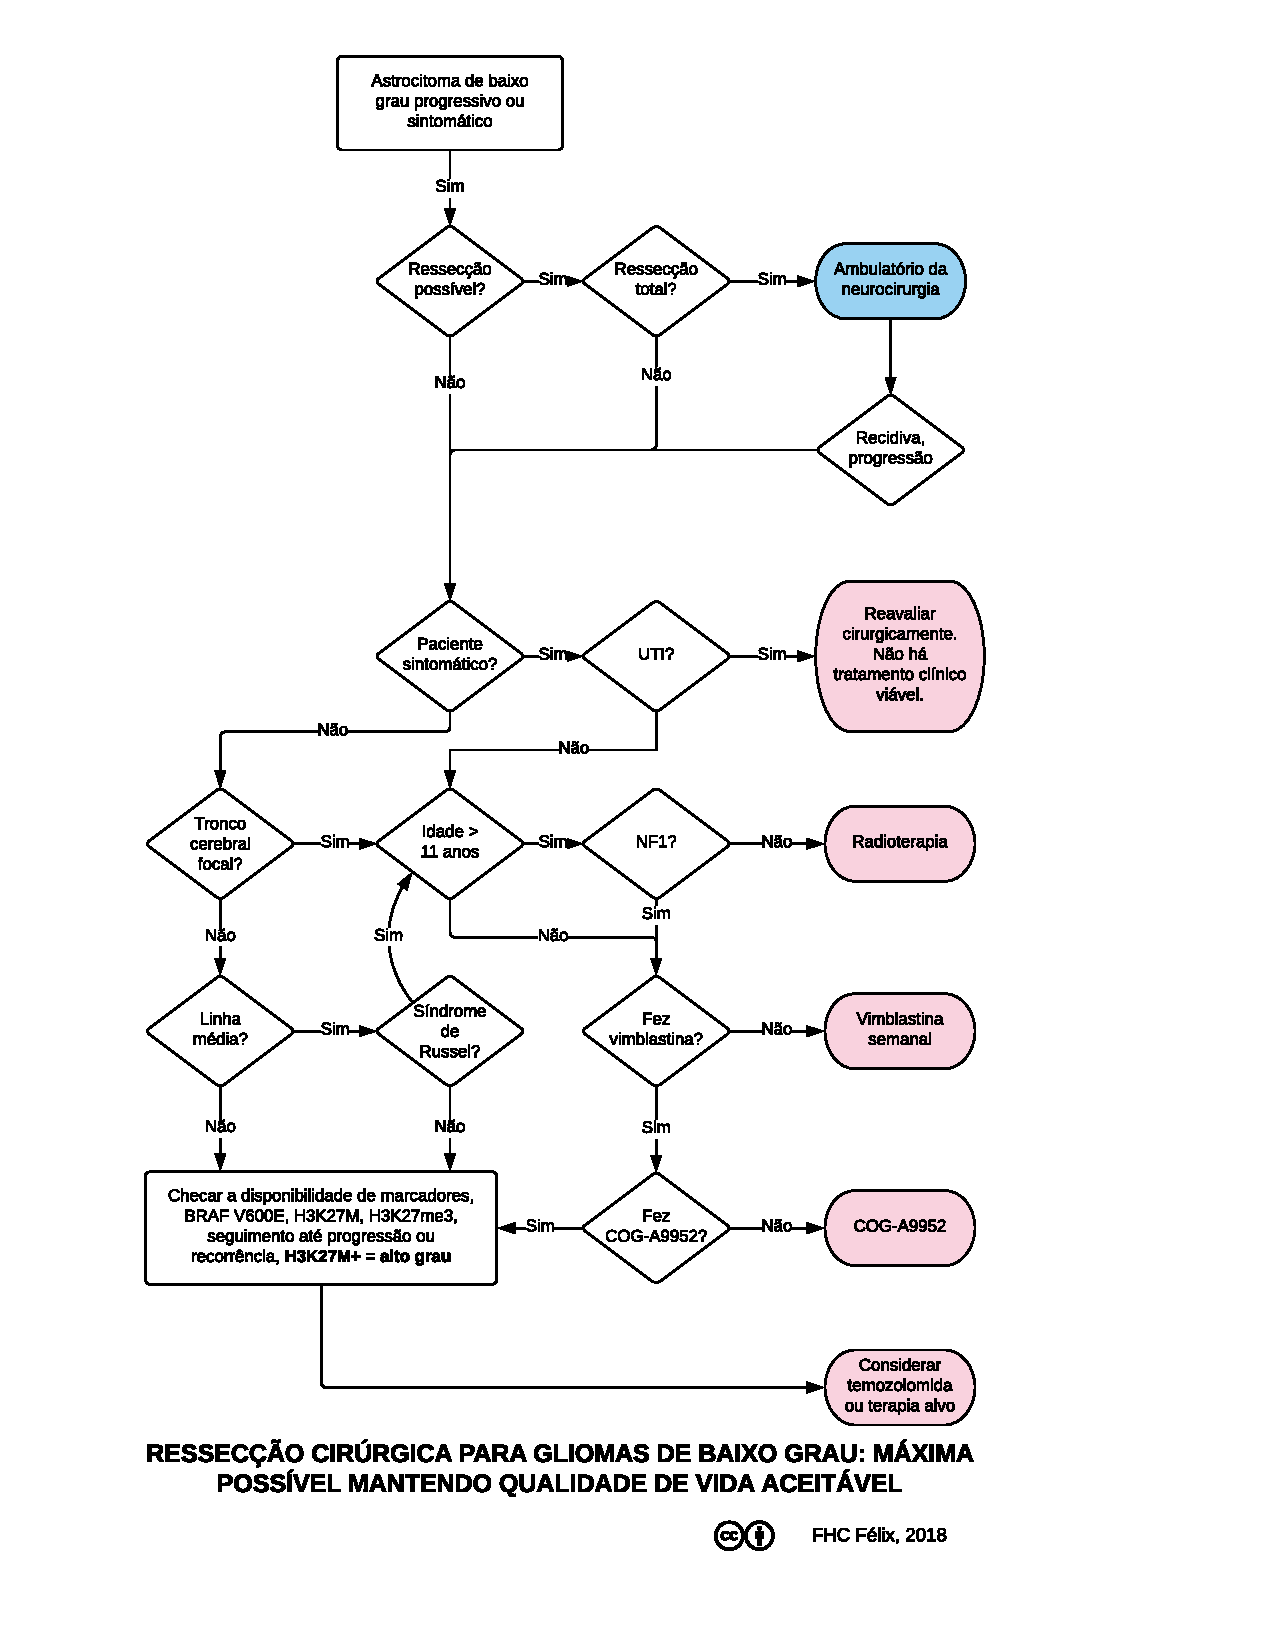
\includegraphics[scale=0.6,trim = 15mm 10mm 45mm 5mm,clip]{fig/fig3.pdf}
\caption{Tratamento de crianças com gliomas e outros tumores neuroepiteliais de baixo grau.}
%\label{Rotulo}
\end{figure}
\end{center}

Esse grupo inclui os astrocitomas, oligodendrogliomas, gangliogliomas e tumores neurogliais mistos ou variantes (grupos IIIa, b e d da CICI 3) \cite{CNCR20910}. A denominação de baixo grau refere-se à classificação da OMS para tumores do sistema nervoso central, a qual divide as neoplasias em 4 grupos, baseada em critérios histológicos. A classificação da OMS para tumores do sistema nervoso central constitui uma “escala de malignidade”, mais do que um esquema de estadiamento convencional \cite{louis}. Os tumores classificados como Grau I ou II são coletivamente denominados tumores de baixo grau de malignidade, enquanto aqueles classificados como Grau III ou IV são designados tumores de alto grau de malignidade. Os tumores de baixo grau são comumente tratados apenas cirurgicamente, com elevados índices de cura e sobrevida prolongada. Tumores astrocíticos e oligodendrogliais de baixo grau têm bom prognóstico associado à ressecção cirúrgica como única terapia. Todavia, a possibilidade de ressecção cirúrgica completa varia muito de acordo com o sítio tumoral \cite{wisof}.

Gliomas cerebelares são passíveis de ressecção completa em \(60-70\%\) dos casos, a maioria são astrocitomas pilocíticos (grau I) e seu comportamento é praticamente benigno \cite{gan}. A recidiva após ressecção e a progressão para tumores de maior grau de malignidade são muito raras. Mesmo tumores incompletamente ressecados mostram uma baixa propensão a progredir. A sobrevida livre de progressão em 5 anos após a cirurgia é de \(84-91\%\). A sobrevida livre de progressão em 5 anos em pacientes com doença residual é de \(54-63\%\) \cite{wisof}. 

Gliomas da via óptica e hipotálamo (e demais tumores diencefálicos ou da linha média) são lesões difusas, infiltrativas, em sua maioria astrocitomas de baixo grau (pilocítico ou difuso), com maior chance de disseminação e metástase no neuro-eixo, com maior incidência em pacientes com neurofibromatose tipo 1. Devido a sua natureza infiltrativa e ao risco de sequelas visuais e neuro-endócrinas, a ressecção cirúrgica não é realizada na maioria dos casos e a biópsia somente está indicada nos casos de imagem atípica. A maioria dos pacientes é tratada com base apenas em imagens sugestivas. Apesar de sua histologia, têm um prognóstico mais reservado do que os pacientes com lesões cerebelares \cite{gan}. A sobrevida livre de progressão em 5 anos é de \(47\%\) \cite{wisof}. 

Oligodendrogliomas, tumores mistos e variantes de tumores astrocíticos são raros em crianças (\(1\%\) ou menos de todos os tumores cerebrais). São tumores da substância branca supratentorial, infiltrativos, e o controle cirúrgico é curativo na maioria. Terapia adjuvante não está bem definida para estes tumores \cite{gan}. A sobrevida livre de progressão em 5 anos é de \(67\%\) \cite{wisof}.

O papel da cirurgia no controle dos gliomas de baixo grau está bem estabelecido. O estudo prospectivo multi-institucional do Children’s Oncology Group (COG) CCG9891 avaliou uma coorte de \(518\) pacientes diagnosticados com tumores de origem glial, tratados inicialmente com ressecção cirúrgica. Ocorreu revisão central da histologia de todos os casos incluídos. Do total, \(64\%\) dos pacientes não tinha evidência de doença residual após a cirurgia, \(20\%\) tinha doença residual limitada (\(< 1,5 cm^3\)) e \(16\%\) tinha doença residual significante (\(> 1,5 cm^3\)). A maioria dos pacientes (\(76\%\)) tinha astrocitoma pilocítico, \(6\%\) astrocitoma difuso, \(8\%\) ganglioglioma e \(10\%\) oligodendroglioma, tumores mistos ou variantes. A maioria dos pacientes (\(73\%\)) tinha 5 anos ou mais. A maioria (\(57\%\)) tinha tumores cerebelares, \(24\%\) de hemisférios cerebrais, \(14\%\) da linha média e \(4\%\) das vias ópticas ou hipotálamo. 

A sobrevida livre de progressão (SLP) em 5 anos de toda a coorte foi de \(80\%\), sendo \(84 \:a\: 91\%\) para tumores cerebelares, \(78\%\) para hemisférios cerebrais, \(65\%\) para a linha média e \(47\%\) para vias ópticas ou hipotálamo (\(p<0,001\)) (nível 2). A SLP em 5 anos foi de \(83\%\) para astrocitomas pilocíticos, \(88\%\) para gangliogliomas, \(66\%\) para astrocitomas difusos e \(67\%\) para outros tumores (\(p=0,64\)) (nível 2). Finalmente, a ressecção cirúrgica completa foi o fator isolado de maior impacto na progressão nesta coorte, \(94\%\) dos pacientes com ressecção completa estavam livres de progressão após 5 anos, enquanto \(59\%\) dos pacientes com doença residual limitada e \(53\%\) dos pacientes com doença residual significante alcançaram sobrevida livre de progressão prolongada (\(p<0,01\)) (nível 2). 

A conclusão é de que a ressecção completa deve ser tentada sempre que possível (ou seja, desde que não acarrete comprometimento funcional) para os pacientes pediátricos com gliomas de baixo grau (nível 4). Além disso, o fato de que mais de \(50\%\) dos pacientes com doença residual não progrediram em 5 anos indica que as intervenções terapêuticas adjuvantes devem ser postergadas até que ocorra progressão objetiva da doença. No entanto, apesar de sua histologia aparentemente benigna, \(44\%\) dos pacientes progrediram mesmo com doença residual muito limitada, o que indica a necessidade de monitorização dos pacientes com ressecção incompleta, independente da quantidade de tumor residual (nível 2) \cite{wisof}.

Fica evidente que um número significativo de pacientes pediátricos com gliomas de baixo grau sofre recidiva após controle cirúrgico ou não pode ter seu tumor ressecado. Nestes casos, indica-se terapia adjuvante com a intenção de evitar a progressão da doença. Vários estudos exploraram a contribuição da radioterapia e quimioterapia no tratamento de gliomas de baixo grau progressivos. 

Um ensaio fase II não controlado estudou \(78\) crianças com gliomas de baixo grau tratadas com radioterapia conformacional. Os pacientes tinham astrocitoma pilocítico (\(n=50\)), tumores de via óptica ou hipotálamo sem biópsia (\(n=13\)), astrocitoma difuso (\(n=4\)), ganglioglioma (\(n=3\)) e oligodendroglioma, tumores mistos ou variantes (\(n=8\)). A maioria dos tumores localizava-se no diencéfalo (\(47\)), \(17\) no cerebelo e \(3\) nos hemisférios cerebrais. Treze pacientes tinham NF-1, \(25\) receberam QT previamente e \(65\) sofreram cirurgia (biópsia ou ressecção incompleta). O tratamento foi indicado nos pacientes sintomáticos na avaliação inicial ou com evidência radiológica de progressão ou, ainda, com uma lesão residual numa área de risco para progressão. Dentre os pacientes cujo tratamento primário foi radioterapia, mais da metade iniciou o tratamento em menos de 90 dias após o diagnóstico. 

A SLP em 5 anos do grupo foi de \(87\%\). Treze pacientes apresentaram progressão com uma mediana de tempo de \(83\) meses. Quatro pacientes apresentaram falha terapêutica, desenvolvendo doença metastática. Não ocorreu diferença digna de nota entre os tipos histológicos (nível 2). Nenhum dos pacientes com NF-1 teve progressão ou malignização. Um paciente da série desenvolveu um glioma de alto grau na região do campo de irradiação, \(78\) meses após o tratamento. A incidência cumulativa de vasculopatia na série foi de cerca de \(5\%\) em 7 anos e o principal fator de risco para esta complicação foi a idade menor que 5 anos (nível 2) \cite{Merchant01082009}. Em relação aos efeitos cognitivos, um declínio de \(10\) pontos de QI foi estimado para crianças com 5 anos de idade ao tratamento, 5 anos após a radioterapia. O risco cumulativo de desenvolver insuficiência tireoidiana foi de \(64\%\) e de deficiência de GH foi de \(49\%\), em 10 anos. A incidência cumulativa de déficit auditivo foi de cerca de \(6\%\) em 10 anos. A presença de NF-1 foi um fator de risco para vasculopatia e déficit cognitivo (nível 2) \cite{Merchant01082009.2}. 

Em conclusão, esta série mostrou inequivocamente que a radioterapia pode controlar adequadamente os gliomas de baixo grau pediátricos não controlados cirurgicamente, com uma elevada proporção de pacientes tendo sobrevida prolongada sem progressão (nível 4). No entanto, isso ocorre às custas de frequentes efeitos colaterais, provavelmente permanentes. A radioterapia para gliomas de baixo grau deve ser evitada em pacientes com menos de 5 anos, devido ao risco de vasculopatia (nível 2). Apesar do risco cumulativo de déficit auditivo ser baixo e do fato do declínio cognitivo ser menor com o avançar da idade, adiar a radioterapia o quanto for possível parece razoável.

Com o intuito de atrasar o início da radioterapia, vários estudos foram realizados com diferentes esquemas de quimioterapia em crianças com gliomas de baixo grau recorrentes ou progressivos. As combinações mais utilizadas foram: carboplatina e vincristina \cite{packer,gnekow}; procarbazina, tioguanina, lomustina e vincristina (TPCV) \cite{prados}; cisplatina e etoposido \cite{mass}.

Packer \textit{et al} trataram \(78\) pacientes até 15 anos (idade média 3 anos, variando de 3 meses a 16 anos) com gliomas de baixo grau confirmados por histologia ou imagem típica, progressivos, reportando \(56\%\) de resposta radiológica objetiva e \(68 \pm 7\%\) de SLP em 3 anos (nível 4). A maioria dos pacientes (\(n=32\)) tinha astrocitoma fibrilar (difuso), \(17\) tinham astrocitoma pilocítico e \(26\) não tinham histologia. A maioria dos pacientes tinha tumores diencefálicos (\(n=58\)), \(12\) tinham no tronco e \(6\) em outros locais. Somente pacientes que sofreram ressecção de \(50\%\) ou menos das lesões foram admitidos. Não ocorreu revisão central de histologia ou imagens. Este ensaio clínico não avaliou se o esquema conseguia adiar o início da radioterapia, principal motivo do tratamento, devido ao curto tempo de seguimento \cite{packer}. 

A carboplatina fora testada pelo Pediatric Oncology Group (POG), comparando com a iproplatina, num ensaio fase II, randomizado. Um grupo de pacientes pediátricos com tumores cerebrais histologicamente verificados, recorrentes ou progressivos, foi avaliado. O subgrupo de pacientes com astrocitoma de baixo grau (\(12\) pacientes, agregando pacientes de um ensaio não randomizado prévio do POG) não mostrou resposta radiológica objetiva, mas a maioria dos pacientes apresentou estabilização prolongada da doença com a carboplatina, o que motivou os pesquisadores a testá-la num grupo maior \cite{fried}. 

Prados \textit{et al}  trataram \(42\) crianças até 18 anos com gliomas de baixo grau histologicamente confirmados (exceto tumores de diencéfalo em pacientes com NF-1 ou de vias ópticas), com doença progressiva, utilizando a combinação TPCV. A SLP foi de \(45\%\) em 3 anos, com mediana de \(2,5\) anos para progressão (nível 4). A maioria dos pacientes tinha astrocitoma pilocítico (\(n=23\)), \(11\) tinham astrocitoma (sem outra especificação), \(6\) não tinham histologia e \(2\) tinham oligodendroglioma ou ganglioglioma. A maioria dos pacientes tinham tumores hipotalâmicos ou quiasmáticos (\(n=33\)), \(4\) talâmicos e \(5\) em outras localizações. A maioria dos pacientes sofreu ressecção parcial ou subtotal. Este esquema foi derivado de experimentos pré-clínicos indicando que a combinação das drogas utilizadas era sinérgica nas células neoplásicas \cite{prados}. 

O ensaio não randomizado HIT-LGG 1996, do grupo de pediatria oncológica dos países de língua alemã (GPOH) utilizou um esquema de carboplatina e vincristina diferente daquele do COG. Um relato do subgrupo com gliomas hipotalâmico-quiasmáticos que recebeu quimioterapia (\(n=123\)) mostrou SLP de \(61\%\) em 5 anos \cite{gnekow} (nível 4). Os resultados completos do ensaio foram publicados em 2012 \cite{gnekow2}. Um total de \(1031\) pacientes foram recrutados, em um braço sem intervenção pós-cirurgia (ressecção total ou parcial, \(n = 668\)), e outro braço (não cirúrgico ou ressecção parcial) estratificado de acordo com a idade para receber vincristina-carboplatina (\(n = 216\)) ou radioterapia/braquiterapia convencional (\(n = 147\)). A idade média foi \(6,9\) anos, \(40\%\) dos pacientes tinha tumores de linha média e \(68\%\) tinha astrocitoma pilocítico. 

A sobrevida livre de eventos (SLE) em 5 e 10 anos relatada foi de \(47\%\) e \(44\%\) para o grupo tratado com quimioterapia e \(65\%\) e \(62\%\) para o grupo tratado com radioterapia. Entre os fatores afetando adversamente o prognóstico foram observados: ressecção cirúrgica imcompleta, idade < 1 ano ou > 11 anos, sítio tumoral de linha média (nível 4 para tratamento e nível 2 para prognóstico). Sessenta e um dos pacientes tratados com quimioterapia receberam radioterapia \(0,3-8,7\) anos após o primeiro tratamento. O ensaio não comparou o braço tratado apenas com cirurgia com aquele tratado com terapia adjuvante \cite{gnekow2}. 

Com o intuito de tentar melhorar estes resultados, a SIOP e o GPOH iniciaram conjuntamente o ensaio SIOP-LGG 2004, o qual terminou de cadastrar pacientes em 2012. Este ensaio randomizado comparou carboplatina e vincristina com carboplatina, vincristina e etoposido \cite{gnekow3}. Um total de \(497\) pacientes com glioma de baixo grau foram randomizados em dois grupos (\(249\) e \(248\)). A sobrevida livre de eventos em 5 anos foi de \(45-46\%\) e a sobrevida global em 5 anos foi de \(89\%\) em ambos os grupos. 

Concluiu-se que a adição de etoposido ao esquema de vincristina e carboplatina não mostrou nenhuma vantagem. Neste ensaio, a síndrome diencefálica e a idade ao diagnóstico foram fatores que afetaram adversamente o prognóstico. Os autores também questionaram o benefício real da quimioterapia para pacientes pediátricos com lesões do sistema óptico, pois neste ensaio não se demonstrou proteção da visão com a quimioterapia. A recidiva ou progressão nas primeiras \(24\) semanas correlacionou-se com elevada probabilidade de morte\cite{gnekow4}.

Em 2002, um grupo italiano relatou um grupo de 34 crianças com gliomas de baixo grau não ressecáveis, a maior parte hipotalâmico-quiasmáticos (\(n=29\)), tratadas com cisplatina e etoposide. Eles mostraram uma SLP de \(78\%\) em 3 anos, com \(11\) pacientes obtendo remissão parcial e 1 completa (nível 4). No entanto, uma quantidade significativa de pacientes apresentou toxicidade auditiva, um efeito colateral conhecido da cisplatina \cite{mass}.

Apesar da aparente superioridade da combinação carboplatina e vincristina, os ensaios tinham grandes diferenças entre si quanto aos diagnósticos histológicos e topográficos dos pacientes, além de diferenças na terapia prévia. Para definir qual o melhor dentre os dois esquemas, um ensaio fase III randomizado foi levado a cabo pelo COG e seus resultados publicados recentemente \cite{Ater20072012}. O estudo avaliou \(274\) pacientes com 10 anos ou menos, com gliomas de baixo grau e com doença residual (mais de \(5\%\) da lesão inicial ou \(1,5 cm^2\)) ou progressiva. Ocorreu revisão central das imagens e da patologia. Pacientes com tumores hipotalâmico-quiasmáticos foram incluídos com base nas imagens. 

A SLP em 5 anos foi de \(45\%\) para todo o grupo, sendo de \(39\%\) para o esquema carboplatina-vincristina e \(52\%\) para o esquema TPCV. Esta diferença não foi significante num teste de log-rank, mas mostrou-se significante num modelo de sobrevida com fração de cura (cure rate model), onde parte desta diferença deveu-se a pacientes com sobrevida prolongada (\(p<0,05\)) (nível 2). O ensaio encontrou dois preditores independentes da SLP: idade (menor risco entre 1 e 5 anos) e doença residual (menor risco se \(<3 cm^2\)) (nível 2).

Em 2016, o grupo de neuro-oncologia pediátrica do Canadá publicou os resultados de um ensaio fase II que testou a monoterapia com vimblastina semanal para pacientes pediátricos com tumores neuroepiteliais de baixo grau progressivos \cite{lassaletta}. Cinquenta e quatro pacientes (idade média 8 anos, variando de 0,7 a 17), a maioria (\(~ 50\%\)) com tumores da linha média anterior (quiasma óptico e hipotálamo) e astrocitoma pilocítico foram tratados com vimblastina semanal. Quarenta e sete pacientes (\(87\%\)) obtiveram pelo menos estabilização da doença. A SLP em 5 anos foi de \(53\%\) (intervalo ce confiança 95\% 41-68). Pacientes com NF-1 (17 pacientes) mostraram melhor sobrevida livre de progressão, \(85\% (IC95 68-100)\), do que pacientes sem NF-1 (\(42\%, IC95 29-60, p = 0.01\)). Não ocorreu diferença em relação à presença de alterações genéticas de BRAF (nível 4).

O resultado destes ensaios deve ser encarado com senso crítico. Apesar de todos os regimes terapêuticos aparentemente terem conseguido adiar a progressão nos pacientes estudados, nenhum estudo comparou os resultados com um grupo controle randomizado ou não. O fato de que o subgrupo com doença residual do ensaio CCG9891 também ter apresentado SLP equivalente indica que se deve ter cautela na indicação de tratamentos adjuvantes. Uma comparação entre os regimes e com um grupo controle não tratado parece estar justificada. Além disso, uma melhor caracterização dos subgrupos onde o tratamento farmacológico tem utilidade é necessário.

\subsection{O panorama molecular dos gliomas de baixo grau}

Até 2016, a classificação dos tumores do sistema nervoso central agregava o conhecimento anátomo-patológico e clínico acumulado em 130 anos de neuropatologia desde o trabalho pioneiro de Santiago de Ramón y Cajal \cite{pinero2014santiago}. Neste ano, a Organização Mundial da Saúde (OMS) publicou a revisão de sua quarta edição da Classificação dos Tumores do Sistema Nervoso Central \cite{Louis2016}. Pela primeira vez, a classificação incluiu dados moleculares oriundos de estudos genômicos empreendidos nos últimos 15 anos, desde a conclusão do Projeto Genoma Humano. Dessa forma, o conhecimento sobre as alterações moleculares mais frequentes em gliomas de baixo grau foram agregadas à avaliação clínico-patológica destes tumores, com valor prognóstico já demonstrado. Este novo conhecimento ainda não originou mudanças na prática clínica, tanto em termos de estratificação de grupos de risco, quanto em relação à terapia. No entanto, isso será somente questão de tempo. Até o momento, acumulam-se relatos de casos publicados mostrando resposta de pacientes com gliomas de baixo grau com alterações moleculares bem definidas à terapia alvo direcionada a estas alterações moleculares. Desa forma, é provável que os ensaios clínicos do futuro passem a estratificar os pacientes de acordo com a classificação molecular e que eles sejam tratados de acordo com medicações sem citotoxidade geral, como os inibidores de tirosina quinase \cite{now209}.

A principal doença desse grupo a ter seu panorama molecular definido também é a mais comum em crianças e adolescentes: astrocitoma piloćitico. Em 2008, foi descrita uma duplicação gênica em tandem no locus 7q34, a qual criava um gene quimérico pela fusão KIAA1549:BRAF em 29 de 44 casos de pacientes com astrocitoma pilocítico. O produto gênico é uma proteína com atividade proteína quinase constitutiva capaz de transformar células gliais \cite{Jones8673}. Essa foi a primeira mutação deste tipo (rearranjo gênico) afetando a via RAS/RAF documentada em um tumor esporádico. Uma avaliação de 64 casos pediátricos de astrocitoma pilocítico mostrou a presença da mutação pontual V600E do gene BRAF em 6 pacientes e uma mutação B-Raf\textsuperscript{insT}(inserção causando duplicação da treonina 599) em mais 2 pacientes\cite{IJC25893}. Somando-se o número de pacientes com astrocitoma pilocítico que comumente têm NF-1 ou fusões mais raras com RAF1, pode-se concluir que cerca de 80-90\% dos pacientes com esse tumor apresentam uma mutação da via MAPK/ERK (\textit{mitogen-activated protein kinase/extracellular signal-regulated kinase}, caracterizando esta via de sinalização celular como crítica para a gênese deste tumor \cite{Jones2012}. Aparentemente, as diversas mutações são mutuamente excludentes no astrocitoma pilocítico, ou seja os pacientes negativos para a fusão KIAA1549:BRAF ou têm o gene não mutado ou BRAF\textsuperscript{V600E} (ou ainda uma outra mutação mais rara de BRAF). O perfil molecular também influencia a localização dos tumores: NF1 e mutações pontuais de BRAF são mais comuns em tumores de linha média, já as fusões envolvendo BRAF ou RAF1 são mais encontradas no cerebelo \cite{Jones2012}. 

A fusão KIAA1549:BRAF nunca foi demonstrada de forma incontroversa em outros gliomas que não o astrocitoma pilocítico, o que parece indicar que é uma alteração genética praticamente exclusiva deste tumor. Isso dá valor diagnóstico importante em casos de dúvida. De fato, a tendência é considerar os raros casos de "outros gliomas" positivos para esta fusão como sendo, na verdade, variantes histológicas incomuns do astrocitoma pilocítico \cite{Jones2012}. Em contraste, a mutação BRAF\textsuperscript{V600E} não é exclusiva de um tipo tumoral apenas, ocorrendo em mairo frequência em casos de melanoma, carcinoma de cólon e de tireóide. Além de uma pequena porcentagem de astrocitomas pilocíticos, essa mutação é encontrada em vários gliomas de baixo grau menos comuns. Uma análise de \(1320\) casos de tumores primários do sistema nervoso central mostrou positividade de BRAF\textsuperscript{V600E} em \(42\) de \(64\) (\(66\%\)) de xantoastrocitomas pleomórficos, 15 de 23 (65\%) de xantoastrocitomas pleomórficos anaplásicos, \(14\) de \(77\) (\(18\%\)) de gangliogliomas e \(9\) de \(97\) (\(9\%\)) de astrocitomas pilocíticos. Neste último tumor, um terço foram detectados em tumores diencefálicos \cite{Schindler2011}. Dessa forma, a via MAPK/ERK de sinalização celular surge como a principal envolvida na gênese dos gliomas de baixo grau de uma forma em geral, especialmente astrocitoma pilocítico, ganglioglioma e xantoastrocitoma pleomórfico.

Outras alterações genéticas têm sido descritas neste grupo de tumores, sendo que uma das mais recentes é a presença de mutações dos genes MYB e MYBL1 no glioma angiocêntrico e astrocitoma difuso \cite{Tatevossian2010}. Uma avaliação genômica de \(91\) tumores neuroepiteliais de baixo grau menos comuns identificou um marcador genético único em \(84\%\) dos casos. Uma fusão MYB-QKI foi identificada em \(87\%\) dos gliomas angiocêntricos e rearranjos envolvendo MYB/MYBL1 foram encontradas em \(41\%\) dos astrocitomas difusos. Esses dados comprovam alterações destes genes como as mais importantes nestes dois tipos de tumores gliais \cite{Qaddoumi2016}. Mutações pontuais de FGFR1 são as mais comuns em gliomas de baixo grau depois da mutação BRAF\textsuperscript{V600E} \cite{now209}. Uma alteração genética de FGFR1, incluindo mutações pontuais, duplicações internas do domínio quinase e fusões foram encontradas em \(82\%\) de DNET (\textit{dysembrioplastic neuroepithelial tumors}) e \(40\%\) de tumores oligodendrogliais, na mesma avaliação genômica.

Fica claro pelos dados de pesquisa genômica associada com clínica nos últimos \(10-15\) anos que as alterações moleculares mais frequentes em tumores neuroepiteliais de baixo grau ocorrem em 3 genes: BRAF, MYB e FGFR1 \cite{now209,Qaddoumi2016}. Outras alterações moleculares descritas parecem girar em torno das vias de sinalização molecular representadas por estes mesmos genes. Isso abre uma nova era de possibilidades para diagnóstico e terapia baseadas em biologia molecular. Os ensaios clínicos do futuro vão rapidamente agregar estes dados para definir subgrupos de prognóstico bem definido e validar o tratamento com terapia-alvo.

\subsection{Questões importantes ainda por responder}

A evidência apresentada até o momento deixa uma série de lacunas em nosso conhecimento sobre o tratamento clínico de tumores neuroepiteliais de baixo grau em crianças e adolescentes. Entre as diversas questões que podemos levantar, algumas podem ser apontadas como mais evidentes:

\begin{enumerate}
\item Pacientes com tumor residual maior que \(1,5 cm^2\) e menor que \(3,0 cm^2\) serão melhor seguidos com conduta expectante? 
\item Para pacientes com mais de 5 anos e mais de \(3,0 cm^2\) de tumor residual, deve-se indicar radioterapia precocemente? 
\item A quimioterapia tem papel restrito aos menores de 5 anos com progressão documentada e naqueles com gliomas hipotalâmico-quiasmáticos? 
\item Deve-se adaptar a estratégia terapêutica de acordo com o sítio tumoral?
\item A vimblastina semanal deve ser a primeira escolha de tratamento quimioterápico?
\item Qual o melhor tratamento após falha terapêutica múltipla (progressão após dois tratamentos com quimioterapia e/ou radioterapia)?
\end{enumerate}

A ausência de ensaios comparativos entre as abordagens terapêuticas e de ensaios com controles não tratados impede a resposta destas questões com certeza. A realização de ensaios clínicos com desenho e poder estatístico para responder estas questões com a maior certeza possível vai exigir uma inédita colaboração internacional, com a participação ativa de centros de tratamento ao redor do mundo. A partir desse esforço, será possível oferecer o melhor e mais eficiente tratamento a todas as crianças e adolescentes com esta patologia.

\subsection{Conclusões}

A conclusão sobre a terapia dos tumores neuroepiteliais de baixo grau é de que, hoje em dia, temos evidência de relativa boa qualidade documentando a história natural deste grupo de tumores, mas a ausência de adequados estudos controlados e randomizados ainda suscita dúvidas quanto à melhor conduta em cada situação. A partir dos dados que temos até o momento, um esquema racional de tratamento para gliomas de baixo grau pediátricos inclui:

\renewcommand{\labelenumi}{\Alph{enumi}}
\begin{enumerate}
\item - A melhor ressecção cirúrgica possível (mantendo ao máximo a função) (nível 2)
\item - Seguimento de todos os pacientes com doença residual (independente da quantidade) (nível 2)
\item - Aguardar a progressão (ou piora sintomática) para indicar terapia adjuvante (mesmo quando doença residual) (nível 2)
\item - Evitar radioterapia em menores de 5 anos e portadores de NF-1 através do uso de quimioterapia (TPCV um pouco superior a carboplatina-vincristina, vimblastina parece ser equivalente) (nível 4)
\item - Tratar com radioterapia lesões progressivas após cirurgia e/ou quimioterapia, em maiores de 8-10 anos (nível 4)
\end{enumerate}

Infelizmente, mesmo com essa abordagem baseada em evidência, uma quantidade significativa de pacientes terá doença progressiva apesar da melhor terapia, mostrando que o tratamento ótimo dos tumores neuro-epiteliais de baixo grau pediátricos ainda não foi atingido. A incorporação de marcadores moleculares e melhor definição de subgrupos de risco devem ser prioridades na agenda da pesquisa clínica.


\bibliographystyle{unsrt}
\bibliography{cpc-neuro2014/bib}

\end{document}
